% == == == == == == == == == == == == == == == ==
%
%   A sample latex file for UoY, Dept. Electronics
%   Lab reports. This is NOT an official document
%   Just some thing I find useful when starting a
%   lab report in latex.
%
%   By  Zak R. A. West, zraw500@york.ac.uk
%
%   Licensed under the GNU GPL v2.0 license
%
% == == == == == == == == == == == == == == == ==

% Use the article class with font size 11pt
\documentclass[12pt]{article}

% Creates placeholder text (Only needed for this example)
\usepackage{blindtext}

% Deal with language and encoding
\usepackage[T1]{fontenc}
\usepackage[utf8]{inputenc}
\usepackage[english]{babel}

% setup page size
\usepackage{geometry}
\geometry{a4paper,margin=1.5in,lmargin=1in,rmargin=1in,headheight=15pt} % reduced margins

% Set up fancy headers and footers
\usepackage{fancyhdr} 
\pagestyle{fancy} % options: empty , plain , fancy
\renewcommand{\headrulewidth}{1pt} % adds line at the bottom of the header

% Set up table of contents
\usepackage[nottoc,notlof,notlot]{tocbibind}
\usepackage[titles,subfigure]{tocloft}

% Set up graphics and figures
\usepackage{graphicx}
\usepackage{wrapfig}
\usepackage{subfig}

% Float images where you want them
\usepackage{float}

% Better tables in latex
\usepackage[table,xcdraw]{xcolor}
\usepackage{booktabs} 
\usepackage{multirow}

% Begin paragraphs with an empty line rather than an indent
\usepackage[parfill]{parskip}

% For including code 
%\usepackage{verbatim}
\usepackage{listings}
\usepackage{color}

% Setup colors for code highlighting
\definecolor{commentcolor}{rgb}{0,0.4,0}
\definecolor{stringcolor}{rgb}{0.5,0.8,0.5}
\definecolor{identifiercolor}{rgb}{0.1,0.1,0.1}
\definecolor{keywordcolor}{rgb}{0.2,0,0.9}

\definecolor{numbercolor}{rgb}{0.5,0.5,0.5}
\definecolor{backgroundcolor}{rgb}{0.975,0.975,0.975}

% Setup style of code listings
\lstset{
	breakatwhitespace=false,
	breaklines=true,
	commentstyle=\itshape\color{commentcolor},
	frame=leftline,
	backgroundcolor=\color{backgroundcolor},
	keepspaces=true,
	keywordstyle=\bfseries\color{keywordcolor},
	identifierstyle=\color{identifiercolor},
	numbers=left,
	numbersep=10pt,
	numberstyle=\small\color{numbercolor},
	rulecolor=\color{black},
	showspaces=false,
	showstringspaces=false,
	showtabs=false,
	stepnumber=1,
	stringstyle=\color{stringcolor},
	tabsize=4,
	title=\lstname
}

% Better maths rendering
\usepackage{array}

% For more list types
\usepackage{paralist}

% Better section formatting
\usepackage{sectsty}

% Sets up formatting for section headings
\allsectionsfont{\sffamily\mdseries\upshape}
\renewcommand{\cftsecfont}{\rmfamily\mdseries\upshape}
\renewcommand{\cftsecpagefont}{\rmfamily\mdseries\upshape}

% Set up header and footer text
\makeatletter
\lhead{\@title}\chead{}\rhead{\@author}
\lfoot{}\cfoot{\thepage}\rfoot{}
\makeatother

% Should show blue underlines on links, but it doesn't appear to work
\usepackage[colorlinks=false, allbordercolors={0 0 0}, linkbordercolor=blue, pdfborderstyle={/S/U/W 1}]{hyperref}

% Tell latex that your images are in a folder called Images
\graphicspath{{Images/}}

% Use url for better url handling
\usepackage{url}

% Use biblatex for citations
\usepackage{csquotes}
\usepackage[
	backend=biber,
	style=numeric,
	sorting=ynt
]{biblatex}
\addbibresource{references.bib}

% My custom title page package
\usepackage{UoYTitlePage}


%%% =====================================================
%%% =====================================================
%%%     You Should Only Have To Edit Stuff Below
%%%     Here. Unless You Want To Change The Style.
%%% =====================================================
%%% =====================================================


% ====================================
% Set up tile, author and other stuff
% ====================================

\uni{University of York}
\dept{Department of Electronics}

\module{Computer Architectures}
\project{Homework Two}

\title{Homework Two}
\author{Y3839090}

\supervisor{ }
\logo{logo}

\abstracttext{
	The second homework assignment for the second year, Computer Architectures module from the Department of Electronics at the University of York.
}

% ====================================
% Start of the main document
% ====================================
\begin{document}

% ============
% Title Page
% ============
\maketitle

% ============
% Contents Page
% ============
\pagenumbering{roman} % Use roman numerals for page numbers
\tableofcontents % Adds a table of contents
\listoffigures % Adds a list of figures
%\newpage
\pagenumbering{arabic} % Use Arabic (integer) numbering

% ============
% Main Pages
% ============
	\section{Question 1}

		\begin{figure}[H]
			\centering
			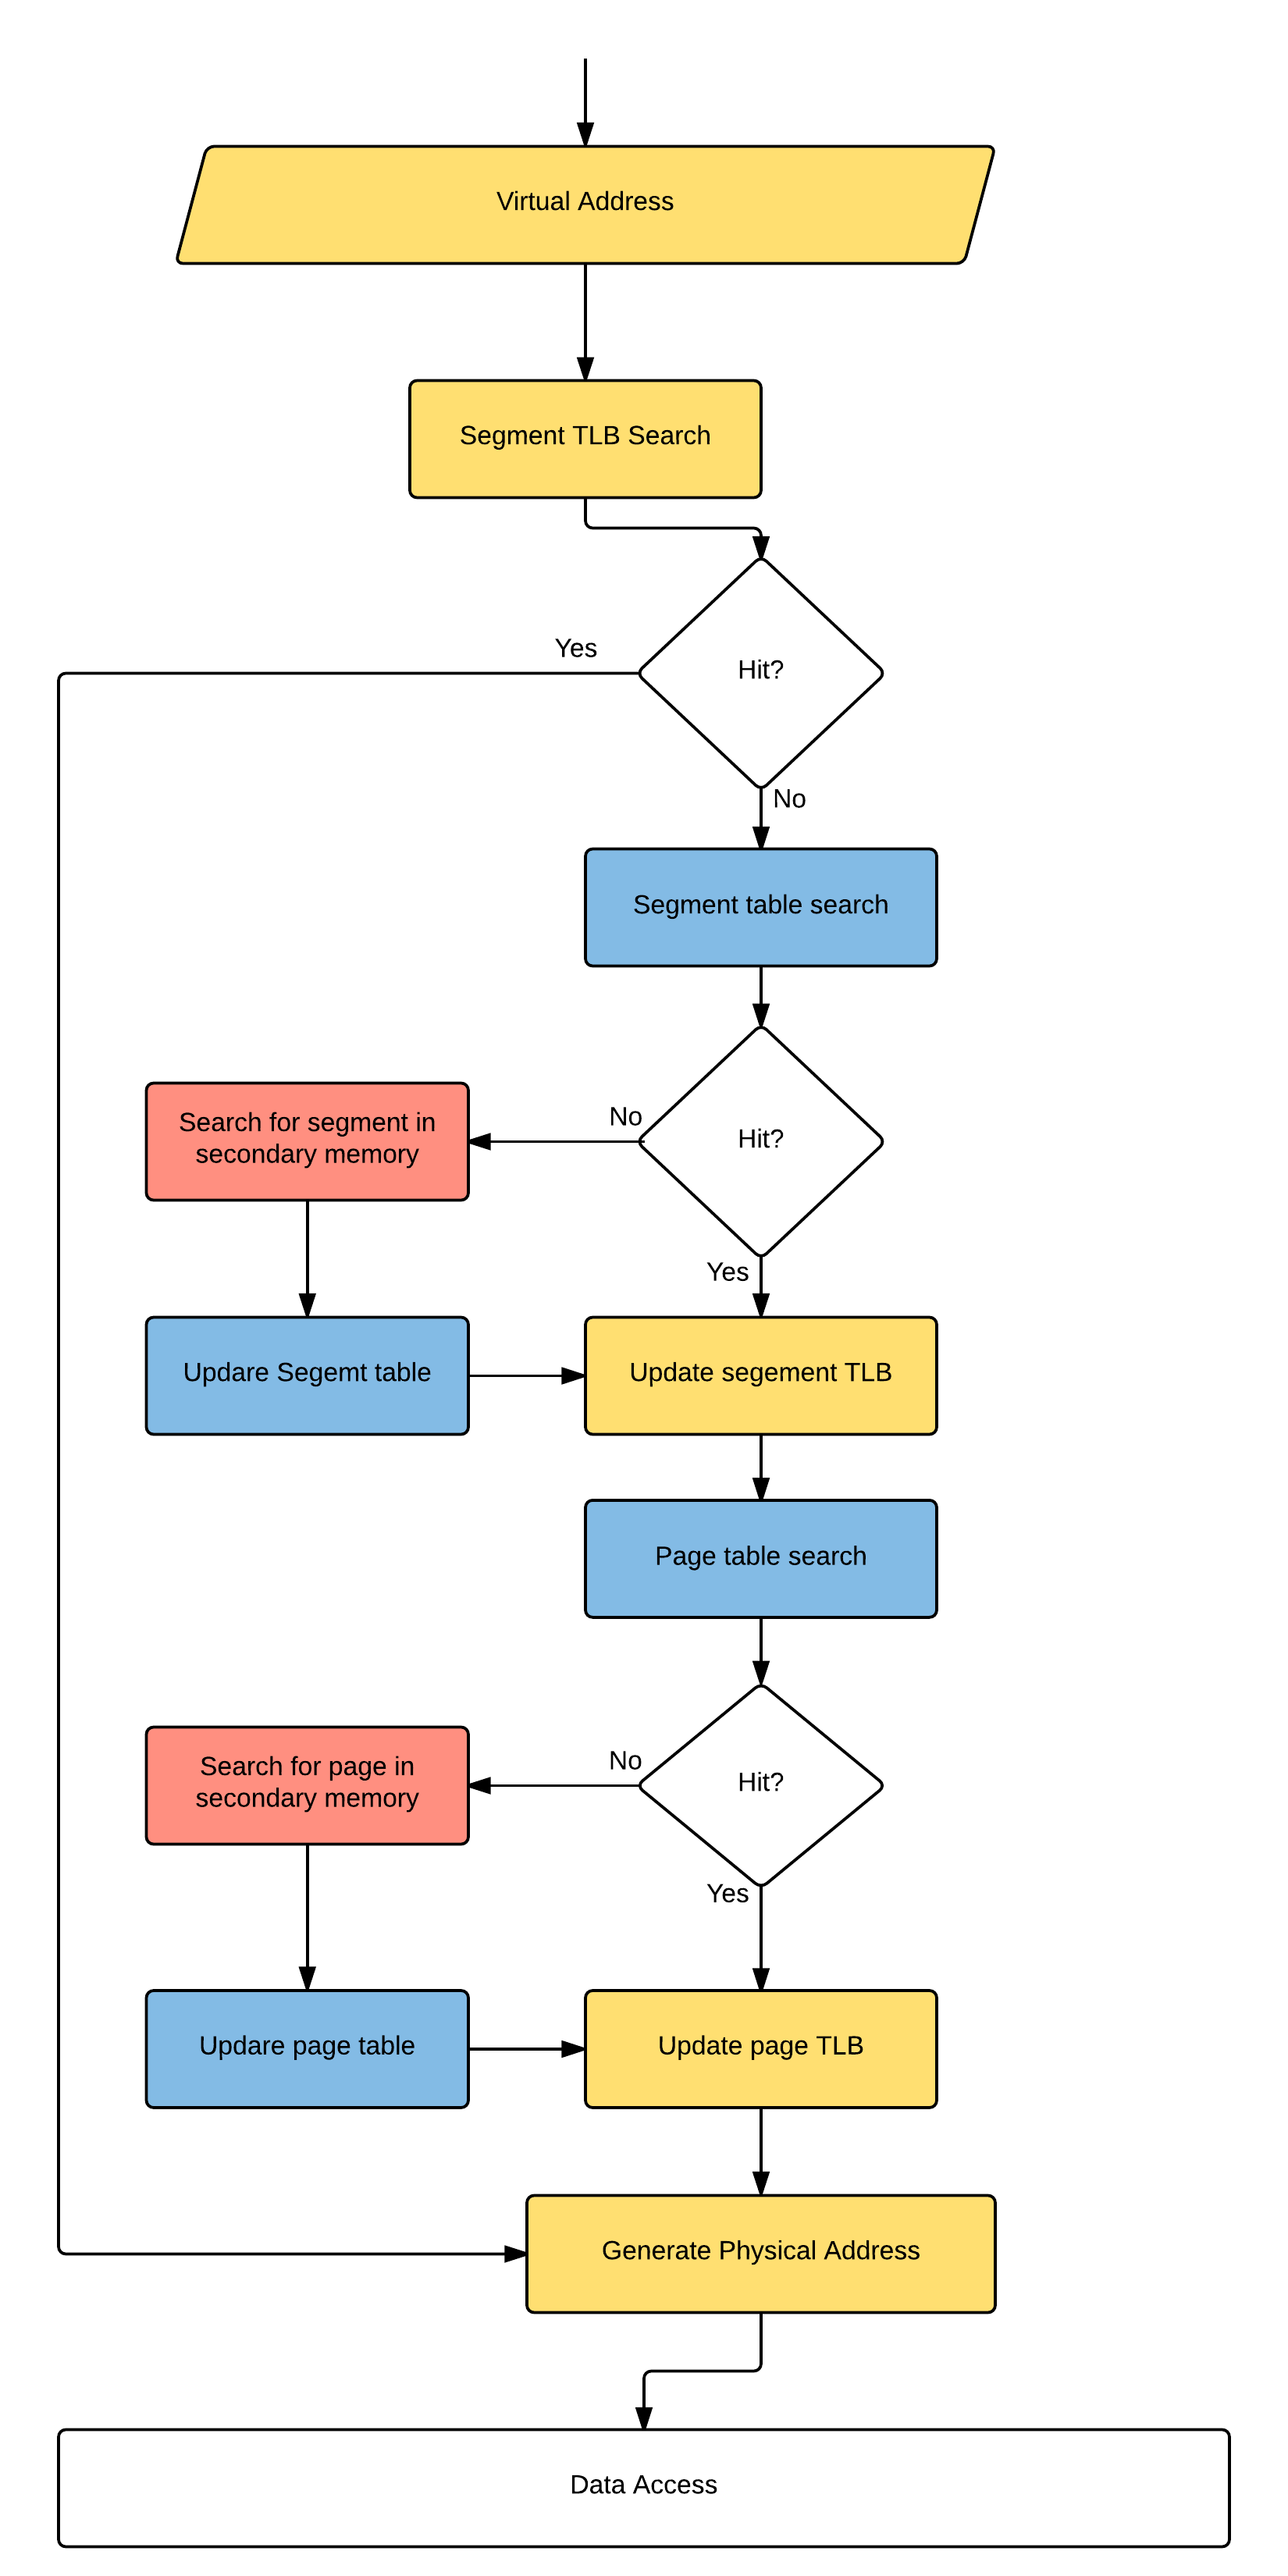
\includegraphics[width=0.6\textwidth]{Paged_Segmentation_Flowchart.png}
			\caption{ A Flowchart of the algorithm for paged segmentation, assuming the presence of separate translation look aside buffers (TLBs) for pages and segments.}
		\end{figure}

		\newpage
	
	\section{Question 2}

		$addresssize = 32 b$

		$blockssize = 64 words = 2048 b$

		$wordsize = 32b$

		$cachesize =  16kB = 131072 b$

		$numblocks = cachesize/blocksize = 64$


		\subsection{direct-mapped cache}

			\subsubsection{sizes}
				\begin{description}
					\item[Offset : ] $size($offset$) = (blocksize B/wordsize B) + wordsize B = (256/32) + 4 = 12b$
					\item[Index : ] $size($index$) = log_2(cachesize/blocksize) - 1 = log_2(16kB/256B) - 1 = 8b$
					\item[Tag : ] $size($tag$) = addresssize- size($offset$) - size($index$) = 32 - 12 - 8 = 12b$
				\end{description}

			\subsubsection{hits and misses}

I used excel to automate find the cache block placement for each of the blocks in the three arrays. From these I was then able to manually work out the total hits and misses.

\begin{table}[H]
\centering
\caption{Table of direct-mapped cache block placement}
\begin{tabular}{lllllll}
\multicolumn{1}{l|}{\multirow{2}{*}{A}}  & \multicolumn{4}{l|}{Block Index}                                       & \multicolumn{2}{l}{Total} \\
\multicolumn{1}{l|}{}                    & 0          & 64         & 128        & \multicolumn{1}{l|}{192}        & Hits       & Misses       \\ \hline
\multicolumn{1}{l|}{majority hit/miss}   & m          & m          & m          & \multicolumn{1}{l|}{m}          & 0          & 256          \\
\multicolumn{1}{l|}{phys addr (byte)}    & 2711684608 & 2711684864 & 2711685120 & \multicolumn{1}{l|}{2711685376} &            &              \\
\multicolumn{1}{l|}{phys block (block)}  & 10592518   & 10592519   & 10592520   & \multicolumn{1}{l|}{10592521}   &            &              \\
\multicolumn{1}{l|}{cache block (block)} & 6          & 7          & 8          & \multicolumn{1}{l|}{9}          &            &              \\
                                         &            &            &            &                                 &            &              \\
\multicolumn{1}{l|}{\multirow{2}{*}{B}}  & \multicolumn{4}{l|}{Block Index}                                       & \multicolumn{2}{l}{Total} \\
\multicolumn{1}{l|}{}                    & 0          & 64         & 128        & \multicolumn{1}{l|}{192}        & Hits       & Misses       \\ \hline
\multicolumn{1}{l|}{majority hit/miss}   & m          & m          & m          & \multicolumn{1}{l|}{m}          & 0          & 256          \\
\multicolumn{1}{l|}{phys addr}           & 2711750144 & 2711750400 & 2711750656 & \multicolumn{1}{l|}{2711750912} &            &              \\
\multicolumn{1}{l|}{phys block}          & 10592774   & 10592775   & 10592776   & \multicolumn{1}{l|}{10592777}   &            &              \\
\multicolumn{1}{l|}{cache block}         & 6          & 7          & 8          & \multicolumn{1}{l|}{9}          &            &              \\
                                         &            &            &            &                                 &            &              \\
\multicolumn{1}{l|}{\multirow{2}{*}{C}}  & \multicolumn{4}{l|}{Block Index}                                       & \multicolumn{2}{l}{Total} \\
\multicolumn{1}{l|}{}                    & 0          & 64         & 128        & \multicolumn{1}{l|}{192}        & Hits       & Misses       \\ \hline
\multicolumn{1}{l|}{majority hit/miss}   & m          & m          & m          & \multicolumn{1}{l|}{m}          & 252        & 4            \\
\multicolumn{1}{l|}{phys addr}           & 3165496832 & 3165497088 & 3165497344 & \multicolumn{1}{l|}{3165497600} &            &              \\
\multicolumn{1}{l|}{phys block}          & 12365222   & 12365223   & 12365224   & \multicolumn{1}{l|}{12365225}   &            &              \\
\multicolumn{1}{l|}{cache block}         & 38         & 39         & 40         & \multicolumn{1}{l|}{41}         &            &             
\end{tabular}
\end{table}
			
				Array A and B map to the same location in the cache and so there is always a cache miss when trying to access one of them. This leads to A and B both having 256 cache misses and 0 cache hits. 

				Array C is mapped to an area in cache that is not occupied by Array A or B and so is cached effectively. It has 4 cache misses and 252 cache hits.

				In total this is 516 cache misses and 252 cache hits.
		\subsection{ fully-associative cache}

			\subsubsection{sizes}
				\begin{description}
					\item[Offset : ] The same as direct mapped cache $ = 12 b$
					\item[Index : ] Fully associative cache dose not have an index $0b$
					\item[Tag : ] $size($tag$) = addresssize- size($offset$) = 32 - 12 = 20b$
				\end{description}

			\subsubsection{hits and misses}
			
				With a fully-associative cache blocks can be placed anywhere this means we avoid the overwriting problems we saw with the direct mapped cache. 

				Each array is 256, 32 bit, words. Giving a total size of exactly 8Kb. The cache is much larger than this (16kB) and so can easily fit all three arrays in cache at once.

				This means that there will only ever be cache misses when a new block of an array needs to be loaded. Since each Array takes up 4 blocks, each array will have 4 cache misses and 252 cache hits 

				In total this is 12 cache misses and 756 cache hits. Which is a big improvement over the direct mapped cache.

		\subsection{set-associative cache with 2 blocks per set with a a not-last-used replacement policy}

			\subsubsection{sizes}
			
				\begin{description}
					\item[Offset : ] The same as direct mapped cache $ = 12 b$
					\item[Index : ] $size($index$) = log_2($numsets$) -1 = log_2($blocksize$/2) -1 = 4$
					\item[Tag : ] $size($tag$) = addresssize- size($offset$) - size($index$) = 32 - 12 -4 = 16b$
				\end{description}

			\subsubsection{hits and misses}

			Again I used excel to help automate the process as mush as possible

\begin{table}[H]
\centering
\caption{Table of set-associative cache with 2 blocks per set with a a not-last-used replacement policy block placement}
\begin{tabular}{lllllll}
\multicolumn{1}{l|}{\multirow{2}{*}{A}}      & \multicolumn{4}{l|}{Block Indexes}                                     & \multicolumn{2}{l}{Total} \\
\multicolumn{1}{l|}{}                        & 0          & 64         & 128        & \multicolumn{1}{l|}{192}        & Miss         & Hit         \\ \hline
\multicolumn{1}{l|}{majority hit/miss}       & m          & m          & m          & \multicolumn{1}{l|}{m}          & 256          & 0           \\
\multicolumn{1}{l|}{phys addr (byte)}        & 2711684608 & 2711684864 & 2711685120 & \multicolumn{1}{l|}{2711685376} &              &             \\
\multicolumn{1}{l|}{phys block (block)}      & 10592518   & 10592519   & 10592520   & \multicolumn{1}{l|}{10592521}   &              &             \\
\multicolumn{1}{l|}{cache Set (set)}         & 6          & 7          & 8          & \multicolumn{1}{l|}{9}          &              &             \\
\multicolumn{1}{l|}{cache Set block (block)} & 0/1        & 0/1        & 0/1        & \multicolumn{1}{l|}{0}          &              &             \\
                                             &            &            &            &                                 &              &             \\
\multicolumn{1}{l|}{\multirow{2}{*}{B}}      & \multicolumn{4}{l|}{Block Indexes}                                     & \multicolumn{2}{l}{Total} \\
\multicolumn{1}{l|}{}                        & 0          & 64         & 128        & \multicolumn{1}{l|}{192}        & Miss         & Hit         \\ \hline
\multicolumn{1}{l|}{majority hit/miss}       & h          & h          & h          & \multicolumn{1}{l|}{h}          & 256          & 0           \\
\multicolumn{1}{l|}{phys addr (byte)}        & 2711750144 & 2711750400 & 2711750656 & \multicolumn{1}{l|}{2711750912} &              &             \\
\multicolumn{1}{l|}{phys block (block)}      & 10592774   & 10592775   & 10592776   & \multicolumn{1}{l|}{10592777}   &              &             \\
\multicolumn{1}{l|}{cache Set (set)}         & 6          & 7          & 8          & \multicolumn{1}{l|}{9}          &              &             \\
\multicolumn{1}{l|}{cache Set block (block)} & 0/1        & 0/1        & 0/1        & \multicolumn{1}{l|}{1}          &              &             \\
                                             &            &            &            &                                 &              &             \\
\multicolumn{1}{l|}{\multirow{2}{*}{C}}      & \multicolumn{4}{l|}{Block Indexes}                                     & \multicolumn{2}{l}{Total} \\
\multicolumn{1}{l|}{}                        & 0          & 64         & 128        & \multicolumn{1}{l|}{192}        & Miss         & Hit         \\ \hline
\multicolumn{1}{l|}{majority hit/miss}       & m          & m          & m          & \multicolumn{1}{l|}{m}          & 256          & 0           \\
\multicolumn{1}{l|}{phys addr (byte)}        & 3165496832 & 3165497088 & 3165497344 & \multicolumn{1}{l|}{3165497600} &              &             \\
\multicolumn{1}{l|}{phys block (block)}      & 12365222   & 12365223   & 12365224   & \multicolumn{1}{l|}{12365225}   &              &             \\
\multicolumn{1}{l|}{cache Set (set)}         & 6          & 7          & 8          & \multicolumn{1}{l|}{9}          &              &             \\
\multicolumn{1}{l|}{cache Set block (block)} & 0/1        & 0/1        & 0/1        & \multicolumn{1}{l|}{0}          &              &            
\end{tabular}
\end{table}

			Although surprising at first this cache does not manage to effectively cache any of the arrays. Because all three of the arrays map top the same cache set, they end up over writing each other due to the cache replacement policy. E.g. If a block of A block 0 of the set, then B goes in position 1. When C is placed into the set it is full so the cache replacement policy is used, and so A is replaced with C. Then we try to access A which is not in the array so there is a miss and B gets overwritten with A. And so on ...
			
			In total there are 768 cache misses and 0 cache hits.

		\subsection{set-associative cache with 8 blocks per set with a least-recently-used replacement}

			\subsubsection{sizes}
			
				\begin{description}
					% TODO:: check these
					\item[Offset : ] The same as direct mapped cache $ = 12 b$
					\item[Index : ] $size($index$) = log_2($numsets$) -1 = log_2($blocksize$/8) - 1 = 2$
					\item[Tag : ] $size($tag$) = addresssize- size($offset$) - size($index$) = 32 - 12 -2 = 18b$
					\item[Sets : ] numSets $=$ numblocks $/$ blocksPerSet $= 64 / 8 = 8 bocks$
				\end{description}

			\subsubsection{hits and misses}
			

\begin{table}[H]
\centering
\caption{Table of set-associative cache with 8 blocks per set with a least-recently-used replacement block placement}
\begin{tabular}{lllllll}
\multicolumn{1}{l|}{\multirow{2}{*}{A}}      & \multicolumn{4}{l|}{Block Index}                                       & \multicolumn{2}{l}{Total} \\
\multicolumn{1}{l|}{}                        & 0          & 64         & 128        & \multicolumn{1}{l|}{192}        & Misses        & Hits       \\ \cline{1-6}
\multicolumn{1}{l|}{majority hit/miss}       & m          & m          & m          & \multicolumn{1}{l|}{m}          & 4             & 252        \\
\multicolumn{1}{l|}{phys addr (byte)}        & 2711684608 & 2711684864 & 2711685120 & \multicolumn{1}{l|}{2711685376} &               &            \\
\multicolumn{1}{l|}{phys block (block)}      & 10592518   & 10592519   & 10592520   & \multicolumn{1}{l|}{10592521}   &               &            \\
\multicolumn{1}{l|}{cache Set (set)}         & 6          & 7          & 0          & \multicolumn{1}{l|}{1}          &               &            \\
\multicolumn{1}{l|}{cache Set block (block)} & 0          & 0          & 0          & \multicolumn{1}{l|}{0}          &               &            \\
                                             &            &            &            &                                 &               &            \\
\multicolumn{1}{l|}{\multirow{2}{*}{B}}      & \multicolumn{4}{l|}{Block Index}                                       & \multicolumn{2}{l}{Total} \\
\multicolumn{1}{l|}{}                        & 0          & 64         & 128        & \multicolumn{1}{l|}{192}        & Misses        & Hits       \\ \hline
\multicolumn{1}{l|}{majority hit/miss}       & m          & m          & m          & \multicolumn{1}{l|}{m}          & 4             & 252        \\
\multicolumn{1}{l|}{phys addr (byte)}        & 2711750144 & 2711750400 & 2711750656 & \multicolumn{1}{l|}{2711750912} &               &            \\
\multicolumn{1}{l|}{phys block (block)}      & 10592774   & 10592775   & 10592776   & \multicolumn{1}{l|}{10592777}   &               &            \\
\multicolumn{1}{l|}{cache Set (set)}         & 6          & 7          & 0          & \multicolumn{1}{l|}{1}          &               &            \\
\multicolumn{1}{l|}{cache Set block (block)} & 1          & 1          & 1          & \multicolumn{1}{l|}{1}          &               &            \\
                                             &            &            &            &                                 &               &            \\
\multicolumn{1}{l|}{\multirow{2}{*}{C}}      & \multicolumn{4}{l|}{Block Index}                                       & \multicolumn{2}{l}{Total} \\
\multicolumn{1}{l|}{}                        & 0          & 64         & 128        & \multicolumn{1}{l|}{192}        & Misses        & Hits       \\ \hline
\multicolumn{1}{l|}{majority hit/miss}       & m          & m          & m          & \multicolumn{1}{l|}{m}          & 4             & 252        \\
\multicolumn{1}{l|}{phys addr (byte)}        & 3165496832 & 3165497088 & 3165497344 & \multicolumn{1}{l|}{3165497600} &               &            \\
\multicolumn{1}{l|}{phys block (block)}      & 12365222   & 12365223   & 12365224   & \multicolumn{1}{l|}{12365225}   &               &            \\
\multicolumn{1}{l|}{cache Set (set)}         & 6          & 7          & 0          & \multicolumn{1}{l|}{1}          &               &            \\
\multicolumn{1}{l|}{cache Set block (block)} & 2          & 2          & 2          & \multicolumn{1}{l|}{2}          &               &           
\end{tabular}
\end{table}

			
				Here A, B and C map to the same set, but there are 8 blocks per set so the current block of all three can be kept in memory at the same time with out overwriting each other.
			
				In total there are 12 cache misses and 756 cache hits.

	\section{Question 3}

        \lstinputlisting[language={[x86masm]Assembler},title={Multiplication Algorithm - Original }]{Code/Question3_orig.txt}
		
		\subsection{RAW Data Hazards Running On Arch D}
		
			This is a five stage pipeline so any accesses to data or branches that depend on data, that was assigned less than five instructions ago are data/control hazards that need to be considered.
		
			\begin{enumerate}
				\item \textbf{Data} line $03$ attempts to use the value in $r30$ which is assigned in line $02$
				\item \textbf{Data} line $05$ attempts to use the value in $r30$ which is assigned in line $02$
				\item \textbf{Data} line $07$ attempts to use the value in $r29$ which is assigned in line $04$
				\item \textbf{Data} line $08$ attempts to use the value in $r4$ which is assigned in line $05$
				\item \textbf{Control} line $09$ attempts to use the value in $r6$ which is assigned in line $08$
				\item \textbf{Control} line $14$ attempts to use the value in $r5$ which is assigned in line $03$

			\end{enumerate}

		\subsection{Eliminating hazards without forwarding}
		
			By moving the instruction that depend only on $r0$ to be the very first instruction we can reduce the time spent in stall substantially. The $ori$ that assigns a value to $r30$ is move to the very top as it is the first register that another instruction depends on. next comes the $xori$ that assigns a value to $r29$ as it is the next register than another value depends on. The instruction that loads a value into $r2$ is an odd one because the value in $r2$ is never used within the multiplication algorithm. This means we can essentially use it as a $nop$ instruction, placing it before the instruction that depends on the value of $r30$.

			\lstinputlisting[language={[x86masm]Assembler},title={Multiplication Algorithm - Eliminated Some Data Hazards Without Forwarding Or Nops}]{Code/Question3_NoForwarding.txt}
			
			Adding a $nop$ before the two $load$ instruction that depend on $r30$ eliminates that data hazard, along with the data hazard with the $addi$ the depends on $r29$.
			
			\lstinputlisting[language={[x86masm]Assembler},title={Multiplication Algorithm - Eliminated Some Data Hazards Without Forwarding, With Nops}]{Code/Question3_NoForwarding_Nops.txt}

		\subsection{Eliminating data hazards with forwarding}
			The data hazard on line $05$ which attempts to use the value in $r30$ which is assigned in line $02$, can be solved by using the $F2$ path. Which connects the Register Write stage to the Execute stage.
			
			The data hazard on line $07$ which attempts to use the value in $r29$ which is assigned in line $04$, can be solved by using the $F1$ forwarding stage. Which connects the Memory Access stage to the Execute stage.
			
			The data hazard on line $08$ which attempts to use the value in $r4$ which is assigned in line $05$, can be solved by using the $F2$ path. Which connects the Register Write stage to the Execute stage.
		
		\subsection{Branch prediction}
		
			It takes $9$ clock cycles to get from line $01$ up to and including line $09$
		
			It will also take $5$ clock cycles for line $15$'s instruction to propagate all the way threw the pipeline.
		
			\subsubsection{Without any form of speculative execution}
			
				If $B1$ is taken then it takes $4 + 3 = 7$ clock cycles to get to $B2$ otherwise it takes $5 + 3 = 8$ clock cycles to get to $B2$.
				
				The assessment states that the $B1$ branch is taken $50\%$ which means that $8$ times it will take $7$ clock cycles and $8$ times it will take $8$ clock cycles. Giving a total of $ 8\times7 + 8\times8 = 56 + 64 = 120$ clock cycles.
			
				If $B2$ is taken then it takes $1 + 3 = 4$ clock cycles to get to $B1$ again otherwise it takes $3$ clock cycles to get to line $15$.
				
				The assessment states that the $B2$ branch is taken $\frac{15}{16}$ times. This gives a total of $15\times4 + 1\times3 = 64$ clock cycles.
			
				Combining all four of these clock cycle counts gives us the number 0of clock cycles the program will take to execute.
				This gives a total of $9 + 120 + 63 + 5 = 197$ clock cycles.
			
			\subsubsection{With speculative execution using static prediction – predict not taken}
			
				If $B1$ is taken then it takes $4 + 3 = 7$ clock cycles (the same as no prediction, because we predicted wrong!), otherwise, if $B1$ is not taken, it takes $5$ clock cycles (Less than no prediction because we predicted right!).
				
				This gives a total of $ 8\times7 + 8\times5 = 56 + 40 = 96$ clock cycles.
				
				If $B2$ is taken then it takes $1 + 3 = 4$ clock cycles to get to $B1$ again otherwise it takes $1$ clock cycles to get to line $15$.
			
				This gives a total of $15\times4 + 1\times1 = 61$ clock cycles.
				
				
				Combining all four of these clock cycle counts gives us the number 0of clock cycles the program will take to execute.
				This gives a total of $9 + 96 + 61 + 5 = 171$ clock cycles.
				
			\subsubsection{With speculative execution using static prediction – predict taken}
			
				If $B1$ is taken then it takes $4$ clock cycles  (Less than no prediction because we predicted right!), otherwise, if $B1$ is not taken, it takes $5 + 3 = 8$ clock cycles(the same as no prediction, because we predicted wrong!).
				
				This gives a total of $ 8\times4 + 8\times8 = 32 + 64 = 96$ clock cycles.
				
				If $B2$ is taken then it takes $1$ clock cycles to get to $B1$ again otherwise it takes $3$ clock cycles to get to line $15$.
			
				This gives a total of $15\times1 + 1\times3 = 18$ clock cycles.
				
				
				Combining all four of these clock cycle counts gives us the number 0of clock cycles the program will take to execute.
				This gives a total of $9 + 96 + 18 + 5 = 128$ clock cycles.
				
			\subsubsection{With speculative execution using static prediction – direction-based prediction}

				Coincidently(which either means I've messed up or you've designed it this way) direction-based speculation gives the same result as predict taken. Because $B1$ branch has the same clock cycle cost in both predict taken and predict not taken modes.
				
				$B1$ has a positive jump so we are using the predict not taken method on it.
				
				If $B1$ is taken then it takes $4 + 3 = 7$ clock cycles (the same as no prediction, because we predicted wrong!), otherwise, if $B1$ is not taken, it takes $5$ clock cycles (Less than no prediction because we predicted right!).
				
				This gives a total of $ 8\times7 + 8\times5 = 56 + 40 = 96$ clock cycles.
				
				$B2$ has a negative jump so we are using the predict taken method on it.
				
				If $B2$ is taken then it takes $1$ clock cycles to get to $B1$ again otherwise it takes $3$ clock cycles to get to line $15$.
			
				This gives a total of $15\times1 + 1\times3 = 18$ clock cycles.
				
				
				Combining all four of these clock cycle counts gives us the number 0of clock cycles the program will take to execute.
				This gives a total of $9 + 96 + 18 + 5 = 128$ clock cycles.
				
% ============
% Bibliography Pages
% ============
\newpage
\printbibliography
\newpage

% ============
% Appendix Pages
% ============
\appendix

\section*{Appendices}
	\addcontentsline{toc}{section}{Appendices}
	\renewcommand{\thesubsection}{\Alph{subsection}}

	% Add appendices here as subsections






\end{document}